\chapter{Hashing}

From linear search, which takes \(O(n)\) time, to binary search, which takes \(O(\log n)\) time, the time is reduced. However, is there another data structure that allows better time? The answer is hashing.

\section{Introduction}
In some applications, fully utilizing the entire array is rare, leading to sparse arrays or sparse matrices. To avoid the multiplication operations required to calculate the index of an entry, we use an access table. This auxiliary table contains values like \(0, n, 2n, 3n, \dots, (m-1)n\). When referencing the rectangular array, the index for entry \([i, j]\) is computed by accessing the value at position \(i\) in the auxiliary table, adding \(j\), and using the resulting position.

A table with index set \(I\) and base type \(T\) can be viewed as a function from \(I\) to \(T\), along with two main operations:

- Table access: Evaluate the function at any index in \(I\).

- Table assignment: Modify the function by changing the value at a specified index in \(I\) to a new value.

Insertion involves adding a new element \(x\) to the index set \(I\) and defining the corresponding value for the function at \(x\). Deletion removes an element \(x\) from the index set \(I\), restricting the function to the resulting smaller domain.

However, array indices are not natural identifiers for the items we want to store, access, and retrieve. This limitation is overcome by using hashing.

\subsection{Hashing}
Hashing is a technique used to perform insertions, deletions, and lookups in constant average time. However, hashing does not efficiently support tree operations that require ordering information among elements. There are three important components of hashing:

1. Hash function: to generate a key; 

2. Hash table: to store the elements; 

3. Collision resolution: to resolve conflicts when two keys hash to the same index. 

A hash table is an abstract data type that allows storing and retrieving elements in \(O(1)\) time. This is true when the indices are known and the value at the target index of a store operation can be discarded. Without a complete set of items, we cannot determine the index of an element in a sorted list.

To solve this problem, we use the item as a key and convert it into unique integers that can be used as array indices. Since the index integer is not known at the entry of an item, it would be helpful if the item itself could be used as a key to index the cell where it will be stored. For example, to store names in an array, rather than assigning arbitrary indices, we can sum the ASCII values of each character in the key (e.g., \(\text{a} = 1, \text{b} = 2, \dots\)).

\subsection{General Idea}
As defined previously, a function that performs the conversion is called a hash function. The conversion process is called hashing, and the storage structure used is called a hash table or scatter-storage.

In general, a hash table is an array of fixed size that contains keys. Each key is associated with a value and mapped to a number in the range \(0\) to \(\text{H\_SIZE} - 1\), placing it in the corresponding cell.

The mapping of keys to indices is done by the hash function, which ideally should be simple to compute and should ensure that distinct keys are placed in different cells. However, this is challenging because there are a finite number of cells and a virtually limitless number of potential keys. Therefore, the goal is to design a hash function that distributes the keys as evenly (uniformly) as possible among the cells.

There are several important issues that need to be addressed, which will be discussed in this chapter:

1. Choosing the hash function.

2. Handling collisions.

3. Handling deletions.

\subsection{Hash Table}
The idea of a hash table is to allow many of the different possible keys that might occur to be mapped to the same location in an array under the action of the index function. This is sometimes referred to as scatter-storage or key-transformation.

A hash function takes a key and maps it to an index in the array. However, two or more records may be mapped to the same location, leading to a collision. Therefore, a collision resolution procedure must be devised to handle this situation.

\section{Hash Function}
\subsection{Analysis}
The two principal criteria in selecting a hash function are that:

1. it should be easy and quick to compute,

2. it should achieve an even distribution of the keys that actually occur across the range of indices.

If the input keys are integers, then simply returning \verb|key mod H_SIZE| is generally a reasonable strategy. For example, \verb|student_ID mod 10000| would be a reasonable strategy. Also, it is usually a good idea to ensure that the table size is prime. When the input keys are random integers, this function is simple to compute and also distributes the keys evenly.

\subsection{Truncation}
Truncation can be done by ignoring part of the key and using the remaining part directly as the index (considering non-numeric fields as their numerical codes). For example, if the keys are eight-digit integers and the hash table has 1000 locations, then the first, second, and fifth digits from the right make the hash function, so that 62538194 maps to 394. Although this method is fast, it often fails to distribute the keys evenly through the table.

\subsection{Folding}
We can also partition the key into several parts and combine the parts in a convenient way (often using addition or multiplication) to obtain the index. For example, we can map 62538194 to \(625 + 381 + 94 = 1100\), which is truncated to 100.

\subsection{Modular Arithmetic}
We can use modular arithmetic to convert the key into the index that we want. We can simply use the ASCII values of all the characters in the string, and then return the \verb|result mod H_SIZE|. 

For example, `abcd' mod \(100 = (64 + 65 + 66 + 67) \% 100 = 62\). 

We can also take only 3 characters and use \verb|hash_val = key[0] + 27*key[1] + 729*key[2]|, and then again return the \verb|hash_val mod H_SIZE|, assuming that the key has at least two characters plus the NULL terminator. If the three characters are random, and the table size is 10007, then we would have a reasonably equitable distribution. However, since English is not random, the percentage of the table being hashed to could be less than expected. 

We can improve the hash function by using \verb|hash_val = hash_val << 5 + *key++|, then returning \verb|hash_val mod H_SIZE|. This hash function involves all the characters in the key by computing:
\[
  \sum_{i = 0}^{\text{keySize - 1}} \text{key[keySize - i]} \times 32^{i},
\]
which follows Horner's Rule.

It is common to not use all the characters in the key, since the length and properties of the key would influence the choice.

\section{Collision Resolution}
Though a hash table is an efficient data structure, there could be cases where different elements share the same index, causing a collision. Thus, we need to handle such collisions, and there are several resolutions.

\subsection{Open Hashing}
The first strategy, commonly known as open hashing or separate chaining, is to keep a list of all elements that hash to the same value.

\begin{minipage}{0.7\textwidth}
To illustrate, we assume that the keys are the first 10 perfect squares, where the hashing function is given by \(\text{hash}(x) = x \mod 10\).\\[5pt]
In open hashing, each node contains a linked list, allowing multiple elements to be stored at the same index.\\[5pt]
We can perform \textbf{find} in open hashing by using the hash function to determine which list to traverse. Then, we traverse this list in the normal manner, returning the position where the item is found.\\[5pt]
To perform \textbf{insertion}, we first traverse the list to check whether the element is already present. If it is a new element, it is inserted either at the front or the end of the list. Often, new elements are inserted at the front, as this is convenient and because recently inserted elements are frequently the most likely to be accessed again soon.\\[5pt]
The \textbf{deletion} routine is straightforward, similar to linked lists. After performing a find operation, we delete the item as we would in a linked list.
\end{minipage}
\begin{minipage}{0.3\textwidth}
\begin{center}
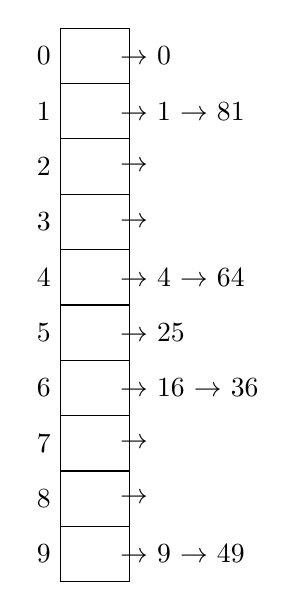
\begin{tikzpicture}
  \coordinate (0);
  \foreach \t/\n[count=\i from 0,evaluate=\i as\j using int(\i+1)] in {
    0/ ,
    1 $\rightarrow$ 81/ ,
    /,
    /,
    4 $\rightarrow$ 64 /,
    25 /,
    16 $\rightarrow$ 36/,
    /,
    /,
    9 $\rightarrow$ 49/
  }
  \node at(\i.south)[anchor=north,draw,minimum height=2em,minimum width=2.5em,outer sep=0pt](\j){\n}
      node at(\j.west)[align=right,left]{\i} 
      node at(\j.east)[align=left,right,xshift=-.7em]{$\rightarrow$ \t};
\end{tikzpicture}
\end{center}
\end{minipage}

The use of linked storage can save a considerable amount of space. It allows for simple and efficient collision handling, and the size of the hash table no longer needs to exceed the number of records we have. Additionally, deletion is faster compared to other methods.

However, all the pointers (links) require space, and even if the number of records is small, the space used is comparatively larger. Thus, it takes longer time to allocate the new cells, and it requires the implementation of another data structure. Thus, we introduce Closed Hashing.

\subsection{Closed Hashing}
In closed hashing, if a collision occurs, alternate cells are tried until an empty cell is found.

For example, cells \(h_0(x), h_1(x), \cdots\) are tried in succession where \(h_i(x) = (\text{hash} + f(i)) \mod \text{H\_SIZE}\), with \(f(0) = 0\).

The function \(f(i)\) is called the collision resolution strategy. Because all the data goes inside the table, a bigger table is needed for closed hashing than for open hashing. Generally, the load factor should be below \(l = 0.5\) for closed hashing.

Again, we want to perform insertion. An array must be declared that will hold the hash table. Then, all locations in the array need to be initialized to show that they are empty. To insert a record, the hash function for the key is first calculated. If the corresponding location is empty, then the record can be inserted. Otherwise, insertion of the new record would not be allowed, which is what we call a collision.

For the find operation, we again calculate the key first. If the desired record is in the corresponding location, then the retrieval has succeeded. Otherwise, we follow the same procedure as for collision resolution, examining all locations until we find the correct record. However, if the position is empty, then no record with the given key is in the table, and the search is thus unsuccessful.

What we haven't discussed yet is the way to resolve collisions. In general, there are three methods.

\subsubsection{Linear Probing}
This is the simplest method to resolve a collision. Starting with the hash address where the collision happens, do a sequential search for the desired key or an empty location. 

\begin{minipage}{0.5\textwidth}
However, data could become clustered in this method. That is, records start to appear in long strings of adjacent positions with gaps between the strings.\\[5pt]
For example, given \(x = 89, 18, 49, 58, 69\), with \(\text{hash}(x) = x \mod 10\), we can perform insertion as shown on the right.\\[5pt]
For values 89 and 18, they can be inserted directly since the corresponding cell for the address is empty. However, when inserting 49, the key value 9 is repeated. Then it finds the next available cell, which in this case would be at position 0. The same applies to 58 and 69.
\end{minipage}
\begin{minipage}{0.5\textwidth}
\begin{table}[H]
  \centering
  \begin{tabular}{c|c|c|c|c|c|c}
      \toprule
        & Empty Table & 89 & 18 & 49 & 58 & 69  \\
    \midrule
      0 &  &  &  & 49 & 49 & 49  \\
      1 &  &  &  &  & 58 & 58  \\
      2 &  &  &  &  &  & 69  \\
      3 &  &  &  &  &  &   \\
      4 &  &  &  &  &  &   \\
      5 &  &  &  &  &  &   \\
      6 &  &  &  &  &  &   \\
      7 &  &  &  &  &  &   \\
      8 &  &  & 18 & 18 & 18 & 18  \\
      9 &  & 89 & 89 & 89 & 89 & 89  \\
      \bottomrule
  \end{tabular}
\end{table}
\end{minipage}

Although they can all be inserted, the time to search for an empty cell may be long. Since the records are not distributed uniformly and become progressively more unbalanced, this leads to the problem of primary clustering. This problem is essentially one of instability. If a few keys happen randomly to be near each other, then it becomes more and more likely that other keys will join the cluster.  

Assuming a very large table and that each probe is independent of the previous probes, the number of probes for a successful search is equal to the number of probes required when the particular element is inserted. When an element is inserted, it is done as a result of an unsuccessful search. We can use the cost of an unsuccessful search to compute the average cost of a successful search. 

Since the fraction of empty cells is \(1 - \lambda\), the number of cells we expect to probe is \(\frac{1}{1 - \lambda}\).

Then, it can be shown that the expected number of probes using linear probing is roughly 
\[
\frac{1}{2} \left( 1 + \frac{1}{(1 - \lambda)^2} \right)
\]
for insertions and unsuccessful searches. It takes roughly 
\[
\frac{1}{2} \left( 1 + \frac{1}{(1 - \lambda)} \right)
\]
for successful searches. Here, \(\lambda\) is the ratio of the number of elements in the hash table to the table size.

This is inefficient since, intuitively, we need to keep probing, which takes longer. As \(\lambda\) increases, the expected number of probes also increases. This issue becomes more significant if the table is expected to be more than half-full. 

Thus, we have quadratic probing.

\subsubsection{Quadratic Probing}
Quadratic probing avoids the primary clustering problem of linear probing. If there is a collision at hash address \(H\), the method called quadratic probing looks in the table at locations \(h + 0, h + 1, h + 4, h + 9, \cdots\), that is, at location \(h + i^2\) for \(i = 0, 1, 2, \cdots\).

\begin{minipage}{0.5\textwidth}
This reduces clustering, but it is obvious that it will not probe all locations in the table. The idea is that if quadratic probing is used and the table size is prime, then a new element can always be inserted if the table is at least half empty. \\[5pt]
Here we use the same example. Now we use quadratic probing instead. After 18 and 89 being inserted, for 49, it goes to \((9 + 1^2) \mod 10 = 0\) since location 9 is occupied, for 58, it goes to \((8 + 2^2) \mod 10 = 2\), and for 69 it goes to \((9 + 2^2) \mod 10 = 3\). \\[5pt]
Note that if the table is even more than half full, insertion could fail. It is also crucial that the table size is a prime number. Otherwise, the number of alternate locations can be severely reduced.
\end{minipage}
\begin{minipage}{0.5\textwidth}
\begin{table}[H]
  \centering
  \begin{tabular}{c|c|c|c|c|c|c}
      \toprule
        & Empty Table & 89 & 18 & 49 & 58 & 69  \\
    \midrule
      0 &  &  &  & 49 & 49 & 49  \\
      1 &  &  &  &  &  &   \\
      2 &  &  &  &  & 58 & 58  \\
      3 &  &  &  &  &  & 69  \\
      4 &  &  &  &  &  &   \\
      5 &  &  &  &  &  &   \\
      6 &  &  &  &  &  &   \\
      7 &  &  &  &  &  &   \\
      8 &  &  & 18 & 18 & 18 & 18  \\
      9 &  & 89 & 89 & 89 & 89 & 89  \\
      \bottomrule
  \end{tabular}
\end{table}
\end{minipage}

Standard deletion cannot be performed in a closed hash table since the cell might have caused a collision to pass it. Simply put, deleting an entry could break the probing chain, causing searches to miss other items. Thus, lazy deletion is required.

In lazy deletion, we delete an entry by placing a special marker or key in the deleted position. This marker indicates that the position is free for future insertions but should not be treated as empty when searching for other items — ensuring the probing sequence remains unbroken.

\subsubsection{Random Probing}
Rather than having the increment depend on the number of probes already made, we can let it be a simple function of the key itself. For example, we could truncate the key to a single character and use its code as the increment.

For random probing, we use a pseudo-random number generator to obtain the increment. The generator should always produce the same sequence when given the same seed. This method is excellent at avoiding clustering, but it is likely to be slower than others.

\subsubsection{Double Hashing}
Another closed hashing method is double hashing. For double hashing, one popular choice is:
\[
f(i) = i \times h_2(x).
\]
We apply a second hash function to \(x\) and probe at distances \(h_2(x), 2h_2(x), \dots\), and so on. However, a poor choice of \(h_2(x)\) could be disastrous. The function must never evaluate to zero, and it needs to ensure that all cells can be probed.  

For instance, the obvious choice \(h_2(x) = x \mod 9\) would not help if 99 were inserted into the input in the previous example. A function such as:
\[
h_2(x) = R - (x \mod R),
\]

\begin{minipage}{0.5\textwidth}
with \(R\) being a prime number smaller than H\_SIZE, works well. One may also perform triple hashing, and so on. \\[5pt]
Again, we perform insertion for \(x = 89, 18, 49, 58, 69\) using double hashing. Here, we have \(h_2(x) = R - (x \mod R)\), with \(R = 7\). \\[5pt]
After inserting 89 and 18, 49 causes a collision. Then we use \(h_2(49) = 7 - (49 \mod 7) = 7\), so it goes to \((7 + 49) \mod 10 = 6\). Inserting 58 also causes a collision, then we have \(h_2(58) = 7 - (58 \mod 7) = 5\), so it goes to \((5 + 58) \mod 10 = 3\). 
\end{minipage}
\begin{minipage}{0.5\textwidth}
\begin{table}[H]
  \centering
  \begin{tabular}{c|c|c|c|c|c|c}
      \toprule
        & Empty Table & 89 & 18 & 49 & 58 & 69  \\
    \midrule
      0 &  &  &  &  &  & 69  \\
      1 &  &  &  &  &  &   \\
      2 &  &  &  &  &  &   \\
      3 &  &  &  &  & 58 & 58  \\
      4 &  &  &  &  &  &   \\
      5 &  &  &  &  &  &   \\
      6 &  &  &  & 49 & 49 & 49  \\
      7 &  &  &  &  &  &   \\
      8 &  &  & 18 & 18 & 18 & 18  \\
      9 &  & 89 & 89 & 89 & 89 & 89  \\
      \bottomrule
  \end{tabular}
\end{table}
\end{minipage}

\subsection{Rehashing}
\begin{minipage}{0.55\textwidth}
There could be cases where the hash table becomes too full, causing the running time for operations to deteriorate, especially when there are too many deletions intermixed with insertions. \\[5pt]
To solve this issue, we can build another table that is about twice as large with an associated new hash function. Then, we scan the entire original hash table, compute the new hash value for each element, and insert it into the new table. This process is known as rehashing. \\[5pt]
For example, for a table of size 7, let \(h(x) = x \mod 7\). After inserting \(x = 13, 15, 24, 6\), we insert 23, which makes the table now 70\% full. Thus, we create a new table with size 17. The new hash function is then \(h(x) = x \mod 17\). The old table is scanned, and elements 6, 23, 24, 13, and 15 are then inserted sequentially. \\[5pt]
The running time is \(O(n)\), which is expensive. Therefore, it should not be done too frequently. This leads us to the concept of extendible hashing.
\end{minipage}
\begin{minipage}{0.15\textwidth}
\begin{table}[H]
  \centering
  \begin{tabular}{|c|c|}
    \hline
      0 & 6 \\ \hline
      1 & 15 \\ \hline
      2 &  \\ \hline
      3 & 24 \\ \hline
      4 &  \\ \hline
      5 &  \\ \hline
      6 & 13 \\ \hline
  \end{tabular}
\end{table}
\end{minipage}
\begin{minipage}{0.15\textwidth}
\begin{table}[H]
  \centering
  \begin{tabular}{|c|c|}
    \hline
      0 & 6 \\ \hline
      1 & 15 \\ \hline
      2 & 23 \\ \hline
      3 & 24 \\ \hline
      4 &  \\ \hline
      5 &  \\ \hline
      6 & 13 \\ \hline
  \end{tabular}
\end{table}
\end{minipage}
\begin{minipage}{0.15\textwidth}
\begin{table}[H]
  \centering
  \begin{tabular}{|c|c|}
    \hline
      0 &  \\ \hline
      1 &  \\ \hline
      2 &  \\ \hline
      3 &  \\ \hline
      4 &  \\ \hline
      5 &  \\ \hline
      6 & 6 \\ \hline
      7 & 23 \\ \hline
      8 & 24 \\ \hline
      9 &  \\ \hline
      10 &  \\ \hline
      11 &  \\ \hline
      12 &  \\ \hline
      13 & 13 \\ \hline
      14 &  \\ \hline
      15 & 15 \\ \hline
      16 &  \\ \hline
      17 &  \\ \hline
  \end{tabular}
\end{table}
\end{minipage}

When the amount of data is too large to fit in main memory and must be stored on disk, we minimize disk access by using a tree. 

In definition, the root of the tree is called the \textit{directory}, and the leaves are called \textit{buckets}. The number of bits used by the root is called the \textit{global depth}, and the \textit{bucket size} is the maximum number of elements that a leaf can contain. 

Suppose that our data consists of several 6-bit integers. With global depth \(D\) equal to 2, the root of the tree contains 4 pointers determined by the leading two bits of the data. Each leaf can hold up to \(m = 4\) elements.

\begin{minipage}{0.5\textwidth}
For example, we have the following tree. To insert 36, we first convert it to binary \(100100_2\). The hash function here is the \(D\) most significant bits (MSBs), which is the 2 MSBs in this case. Since the bucket of \(00\) is full, and the global depth is equal to the bucket depth, the directory is split, and the roots now have \(D = 3\). \\[3pt]
Then, we update the content by inserting \(100100_2\) into the directory \(100\). Note that for the same bucket, there could be more than one pointer pointing to it. \\[3pt]
Next, to insert \(000000_2\), we again encounter a collision. However, since the global depth is now larger than the bucket depth, the bucket itself is split instead of the directory. The element can then be inserted.
\end{minipage}
\begin{minipage}{0.5\textwidth}
\begin{figure}[H]
  \centering
  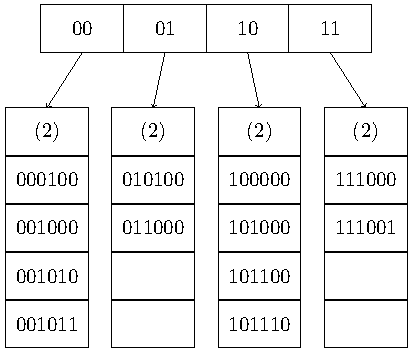
\includegraphics[width=0.8\textwidth]{Figure/EH2.pdf}
  \caption{Original}
\end{figure}
\end{minipage}

\begin{center}
\begin{minipage}{0.48\textwidth}
\begin{figure}[H]
  \centering
  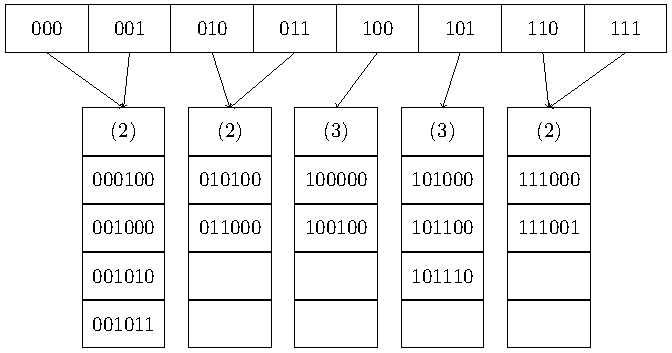
\includegraphics[width=\textwidth]{Figure/EH3.pdf}
  \caption{Insertion 100100}
\end{figure}
\end{minipage}\quad
\begin{minipage}{0.48\textwidth}
\begin{figure}[H]
  \centering
  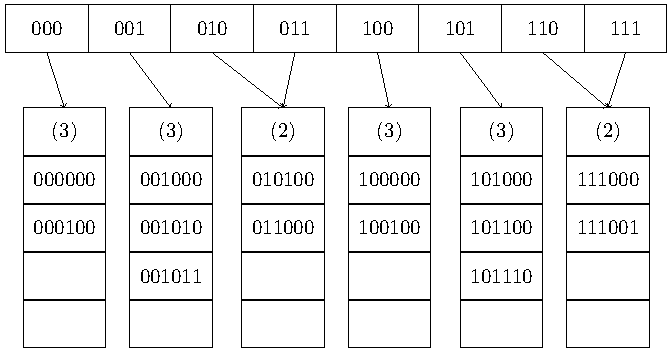
\includegraphics[width=\textwidth]{Figure/EH4.pdf}
  \caption{Insertion 000000}
\end{figure}
\end{minipage}
\end{center}

It is possible that several directory splits will be required if the elements in a leaf agree in more than \(D + 1\) leading bits, i.e., overflow. For example, to insert \(111010_2, 111011_2, 111100_2\), the directory size must be increased to 4. 

This algorithm does not work when there are more than \(m\) duplicates. It is important for the bits to be fairly random. 

In summary, hash tables can be used to implement the insertion and find operations in constant average time. It is especially important to pay attention to details such as the load factor when using hash tables. The choice of hash function is also crucial, especially when the key is not a short string or integer. 

For open hashing, the load factor should be 1, meaning all the cells can be filled. For closed hashing, the load factor should not exceed 0.5, unless unavoidable. It is not possible to find the minimum or maximum since there is no sorting order. 

In applications, hash tables can be used in compilers to keep track of declared variables in source code. They are useful for any graph theory problem where nodes have real names instead of numbers. Additionally, hash tables are commonly used in programs that play games or even online spelling checkers.
